\newpage
\appendix
\counterwithin{figure}{section}

\section{Appendix}

\begin{figure}[h!]
  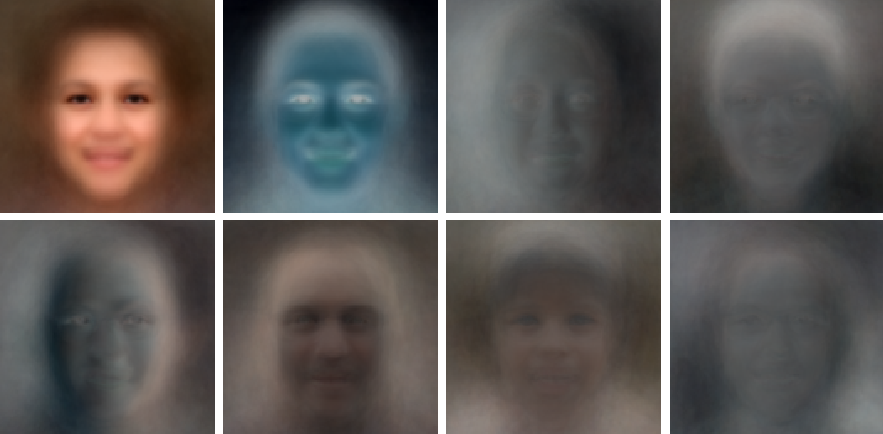
\includegraphics[width=\textwidth]{fig/PCA/pca}
  \caption{Eigenfaces of the FFHQ dataset.}
  \label{eigenface}
\end{figure}

\begin{figure} [h!]
    \centering
    \begin{subfigure}[b]{\textwidth}
        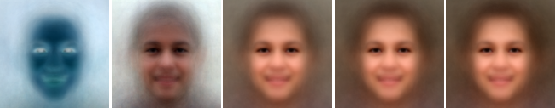
\includegraphics[width=\textwidth]{fig/PCA/pca0}
   
    \end{subfigure}
    \begin{subfigure}[b]{\textwidth}
        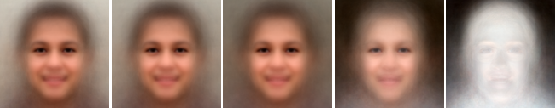
\includegraphics[width=\textwidth]{fig/PCA/pca1}
       
    \end{subfigure}
    \begin{subfigure}[b]{\textwidth}
        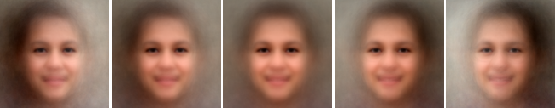
\includegraphics[width=\textwidth]{fig/PCA/pca2}
       
    \end{subfigure}
    \begin{subfigure}[b]{\textwidth}
        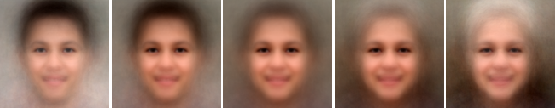
\includegraphics[width=\textwidth]{fig/PCA/pca3}
       
    \end{subfigure}
    \begin{subfigure}[b]{\textwidth}
        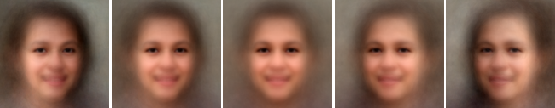
\includegraphics[width=\textwidth]{fig/PCA/pca4}

    \end{subfigure}
    \begin{subfigure}[b]{\textwidth}
        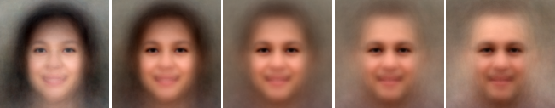
\includegraphics[width=\textwidth]{fig/PCA/pca5}

    \end{subfigure}
    \caption{Synthetic faces created by varying a single principal component to the mean face if the FFHQ dataset. The rows correspond to the principal components such that the first row is the first compoment and so on. }
    \label{pca-components}
\end{figure}

%% VAE
\begin{figure}[h!]
    \centering
    \begin{subfigure}[b]{0.45\textwidth}
        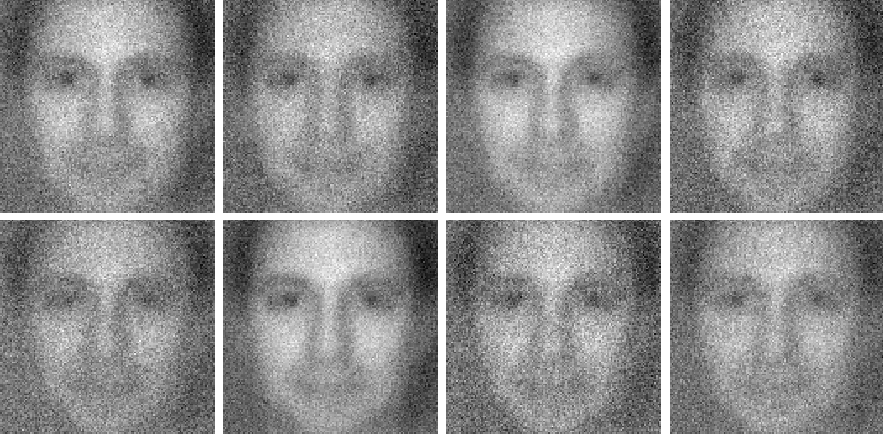
\includegraphics[width=\textwidth]{fig/vae/caltech_epoch50}
        \caption{Epoch 50}
    \end{subfigure}
    ~
    \begin{subfigure}[b]{0.45\textwidth}
         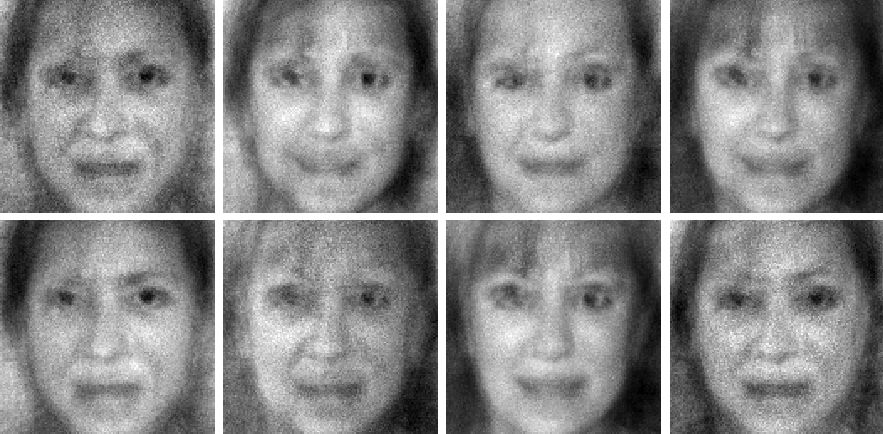
\includegraphics[width=\textwidth]{fig/vae/caltech_epoch400}
        \caption{Epoch 400}
    \end{subfigure}

    \begin{subfigure}[b]{0.45\textwidth}
         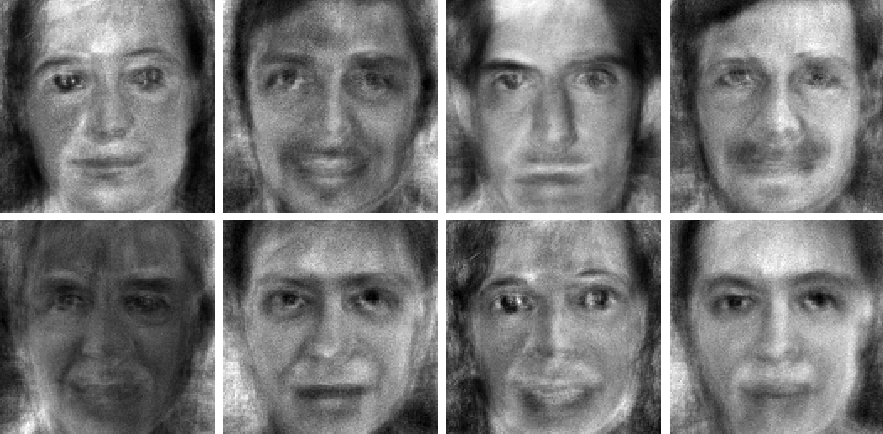
\includegraphics[width=\textwidth]{fig/vae/caltech_epoch1000}
        \caption{Epoch 1000}
    \end{subfigure}
    ~
    \begin{subfigure}[b]{0.45\textwidth}
         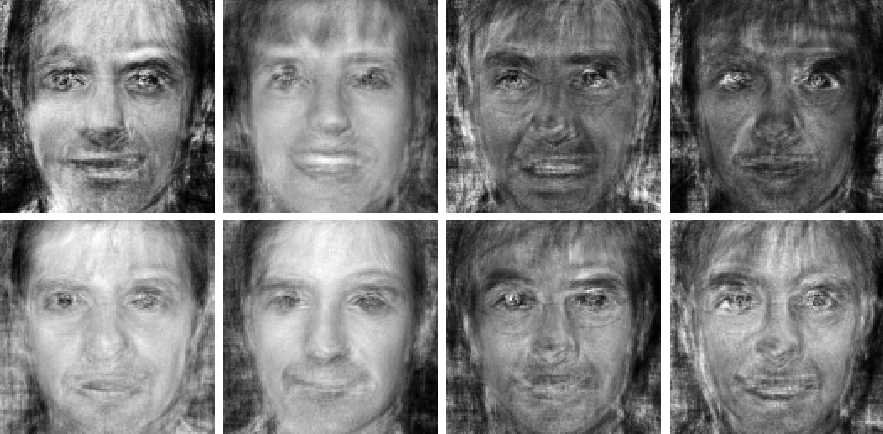
\includegraphics[width=\textwidth]{fig/vae/caltech_epoch2000}
        \caption{Epoch 2000}
    \end{subfigure}

    \begin{subfigure}[b]{\textwidth}
         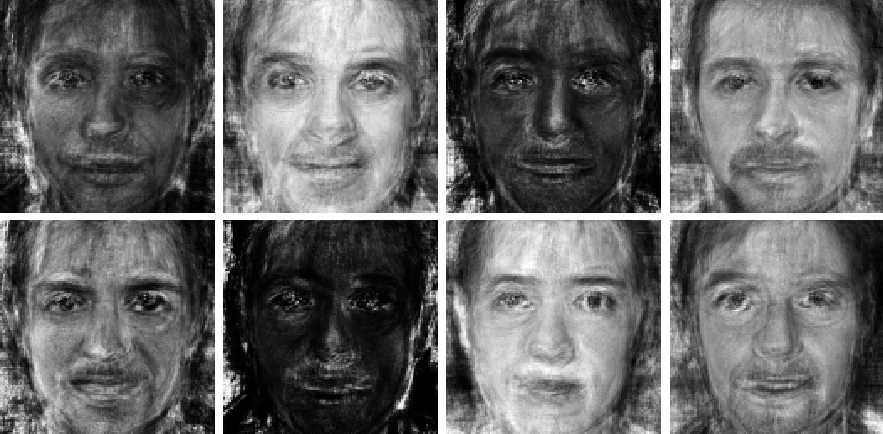
\includegraphics[width=\textwidth]{fig/vae/caltech_epoch4000}
        \caption{Epoch 4000}
    \end{subfigure}
    \caption{Samples from Variational Autoencoder  during training on a black and white version of the Caltech dataset}
    \label{vaq-bwcaltech-samples}
\end{figure}

\begin{figure}[h!]
    \centering
    \begin{subfigure}[b]{0.45\textwidth}
        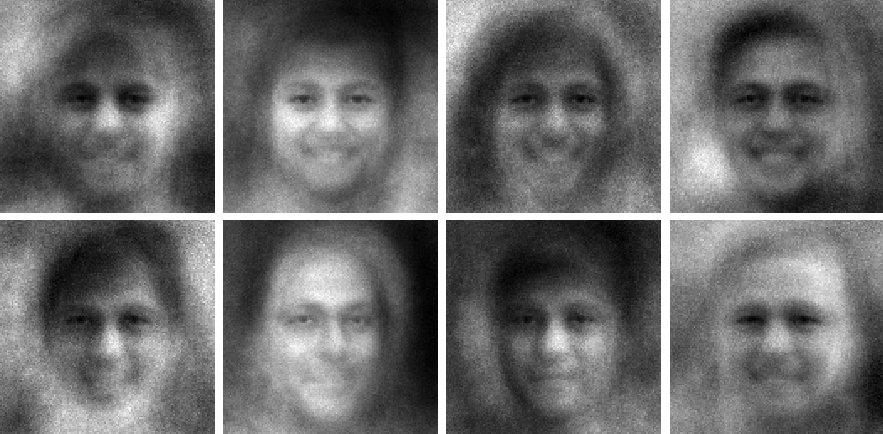
\includegraphics[width=\textwidth]{fig/vae/ffhq_epoch50}
        \caption{Epoch 50}
    \end{subfigure}
    ~
    \begin{subfigure}[b]{0.45\textwidth}
         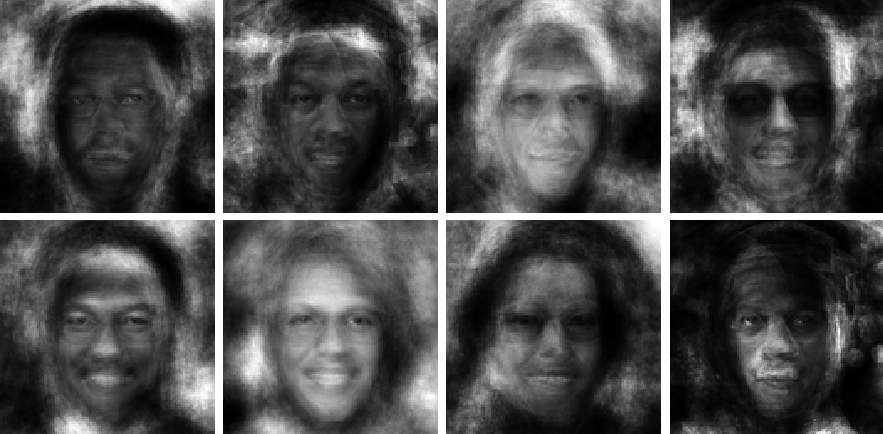
\includegraphics[width=\textwidth]{fig/vae/ffhq_epoch400}
        \caption{Epoch 400}
    \end{subfigure}

    \begin{subfigure}[b]{0.45\textwidth}
         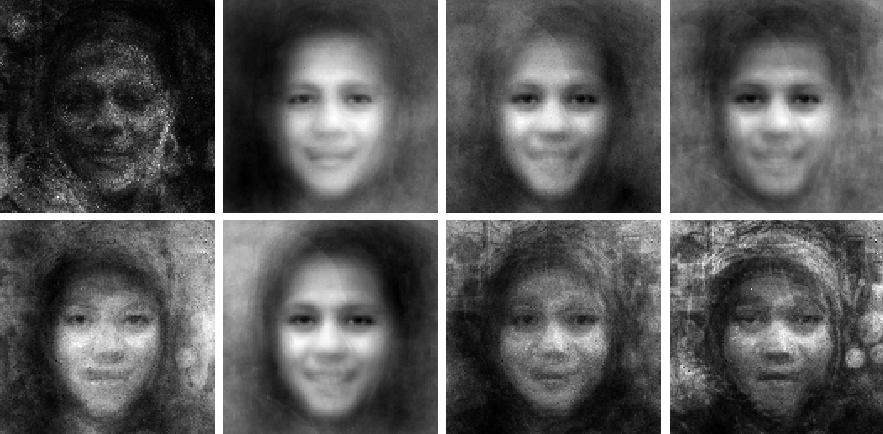
\includegraphics[width=\textwidth]{fig/vae/ffhq_epoch1000}
        \caption{Epoch 1000}
    \end{subfigure}
    ~
    \begin{subfigure}[b]{0.45\textwidth}
         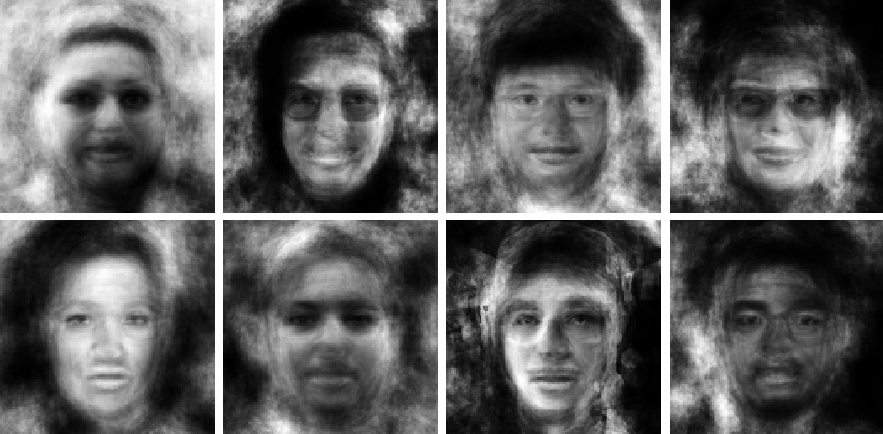
\includegraphics[width=\textwidth]{fig/vae/ffhq_epoch2000}
        \caption{Epoch 2000}
    \end{subfigure}

    \begin{subfigure}[b]{\textwidth}
         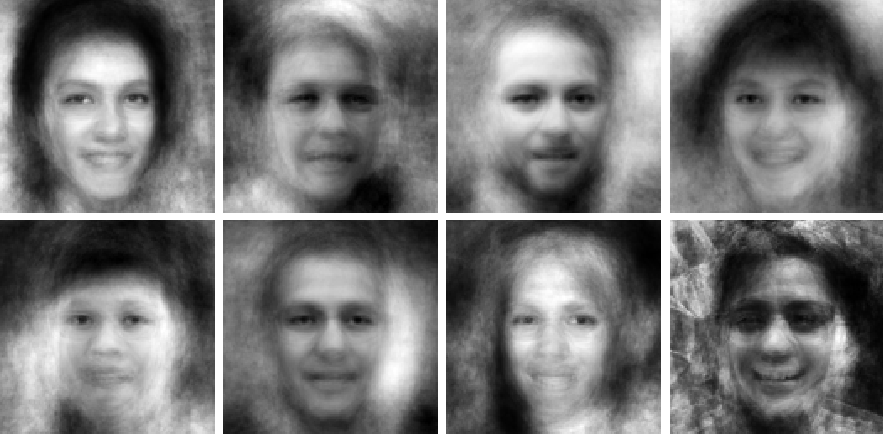
\includegraphics[width=\textwidth]{fig/vae/ffhq_epoch4000}
        \caption{Epoch 4000}
    \end{subfigure}
    \caption{Samples from Variational Autoencoder  during training on a black and white version of  the FFHQ dataset}
    \label{vaq-bwffhq-samples}
\end{figure}

\begin{figure}[h!]
    \centering
    \begin{subfigure}[b]{0.45\textwidth}
        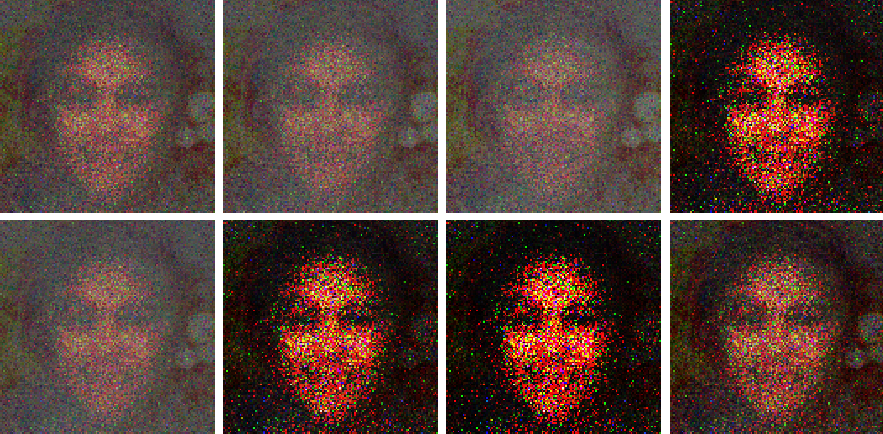
\includegraphics[width=\textwidth]{fig/vae/ffhq_epoch50color}
        \caption{Epoch 50}
    \end{subfigure}
    ~
    \begin{subfigure}[b]{0.45\textwidth}
         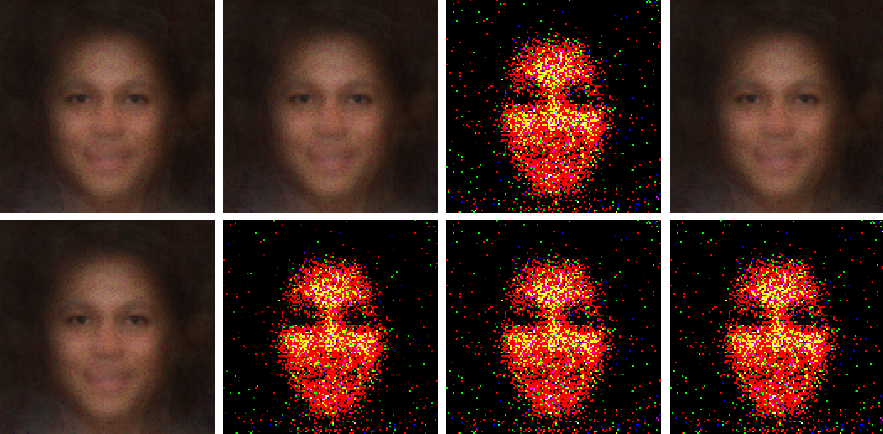
\includegraphics[width=\textwidth]{fig/vae/ffhq_epoch400color}
        \caption{Epoch 400}
    \end{subfigure}

    \begin{subfigure}[b]{0.45\textwidth}
         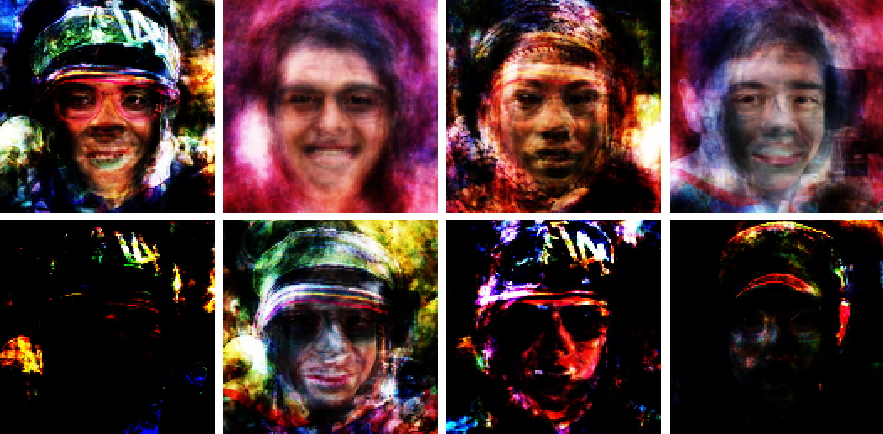
\includegraphics[width=\textwidth]{fig/vae/ffhq_epoch1000color}
        \caption{Epoch 1000}
    \end{subfigure}
    ~
    \begin{subfigure}[b]{0.45\textwidth}
         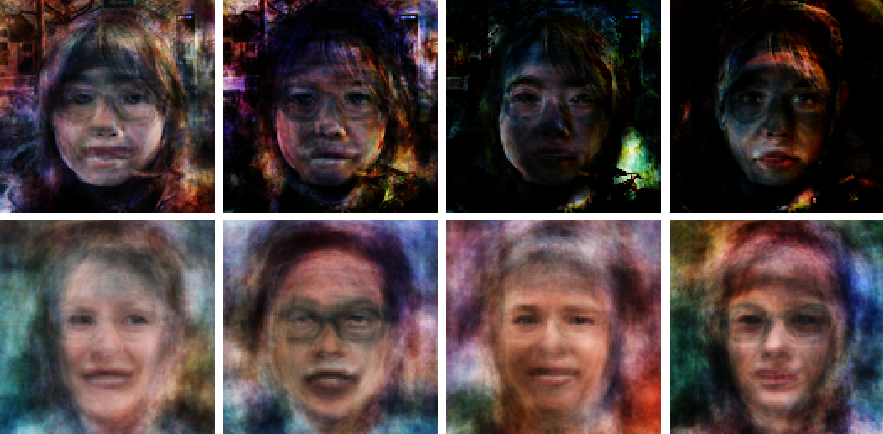
\includegraphics[width=\textwidth]{fig/vae/ffhq_epoch2000color}
        \caption{Epoch 2000}
    \end{subfigure}

    \begin{subfigure}[b]{\textwidth}
         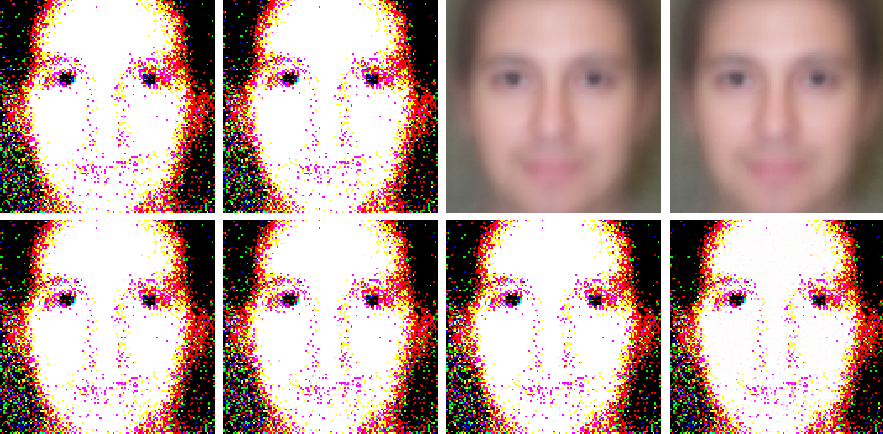
\includegraphics[width=\textwidth]{fig/vae/ffhq_epoch4000color}
        \caption{Epoch 4000}
    \end{subfigure}
    \caption{Samples from Variational Autoencoder during training on the color version of the FFHQ dataset}
    \label{vaq-ffhq-samples}
\end{figure}



%% DCGAN
\begin{figure}
    \centering
    \begin{subfigure}[b]{0.45\textwidth}
        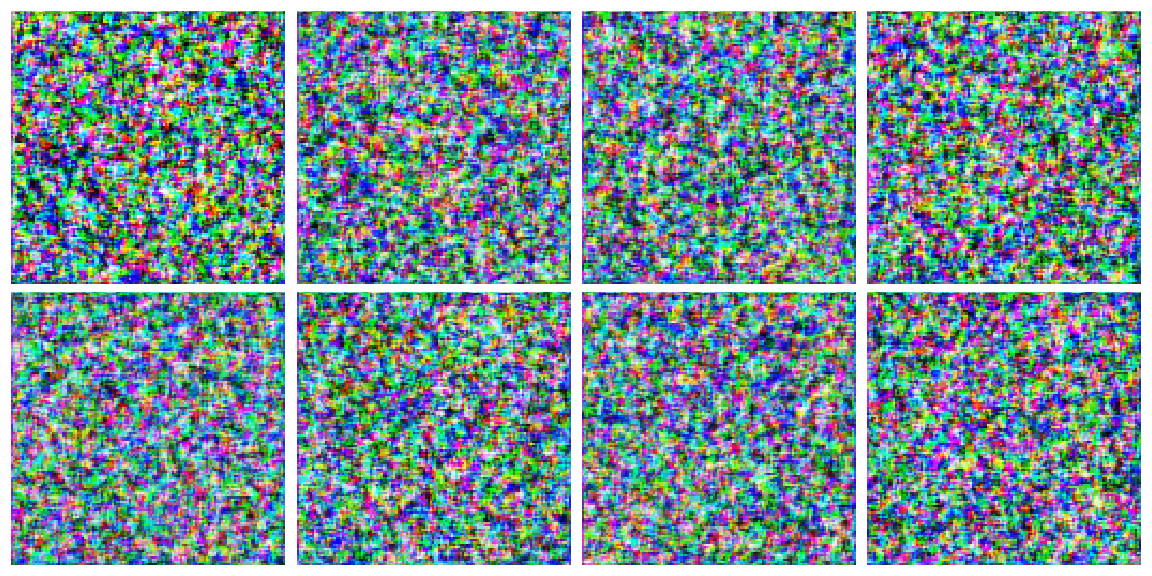
\includegraphics[width=\textwidth]{fig/dcgan/ffhq/epoch0}
        \caption{Epoch 0}
    \end{subfigure}
    ~
    \begin{subfigure}[b]{0.45\textwidth}
        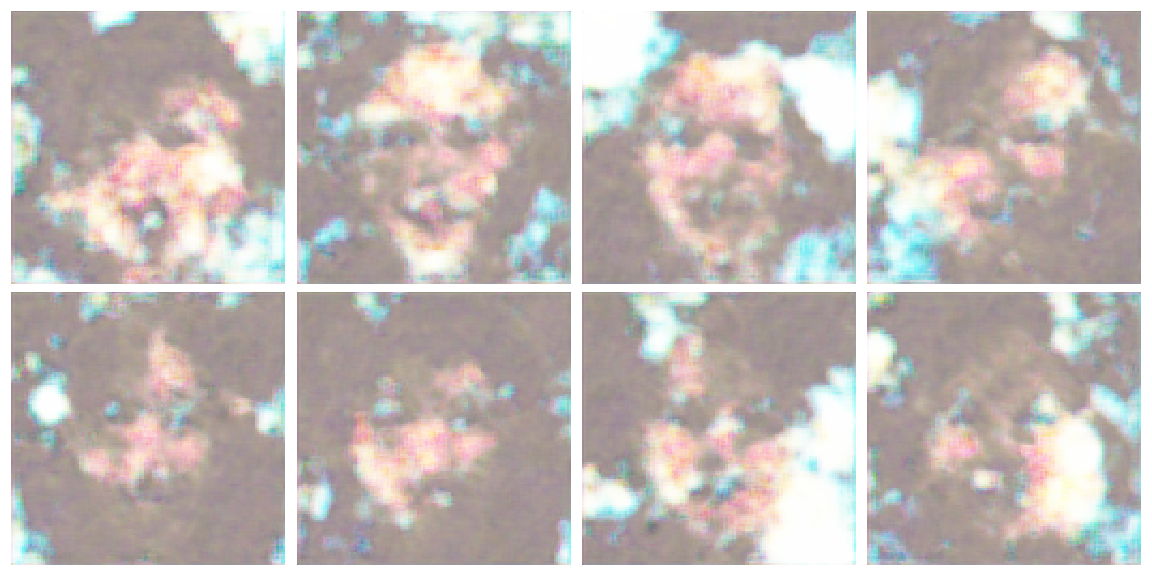
\includegraphics[width=\textwidth]{fig/dcgan/ffhq/epoch200}
        \caption{Epoch 200}
    \end{subfigure}

    \begin{subfigure}[b]{0.45\textwidth}
        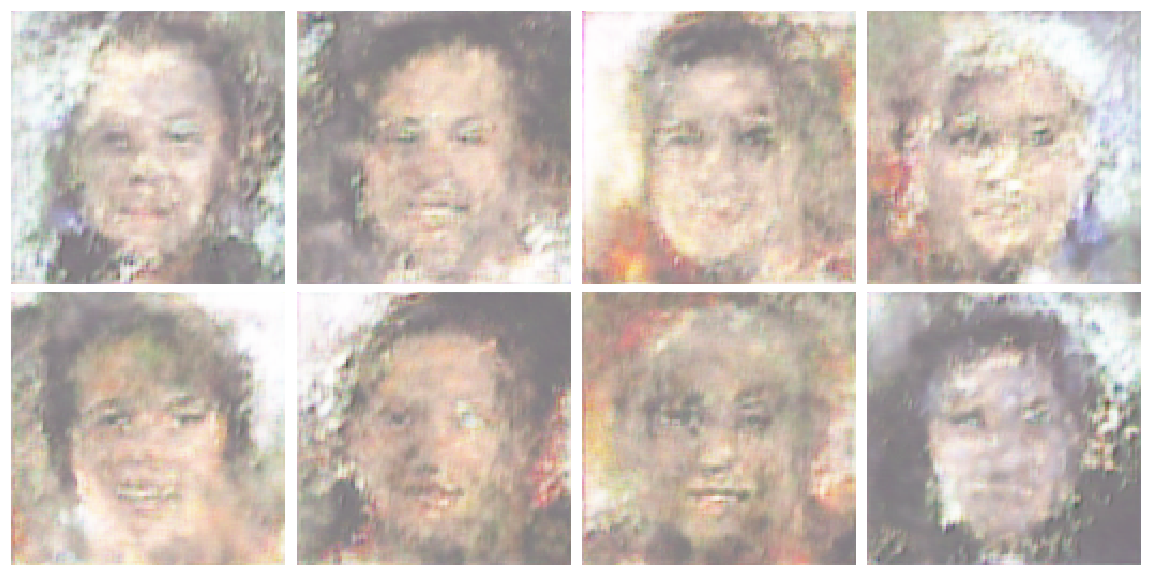
\includegraphics[width=\textwidth]{fig/dcgan/ffhq/epoch2000}
        \caption{Epoch 2000}
    \end{subfigure}
    ~
    \begin{subfigure}[b]{0.45\textwidth}
        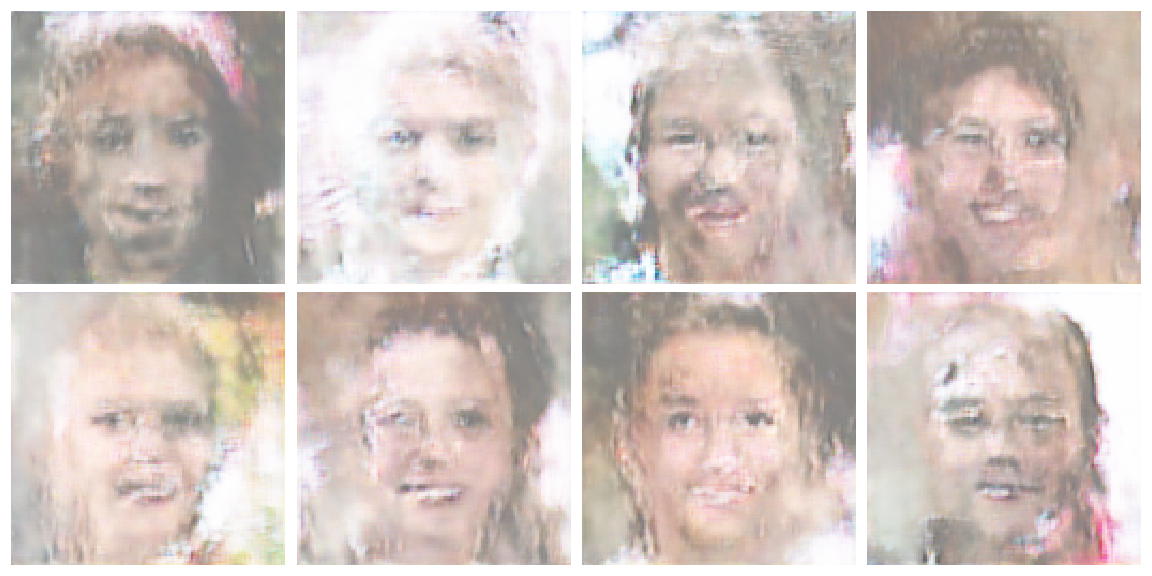
\includegraphics[width=\textwidth]{fig/dcgan/ffhq/epoch4000}
        \caption{Epoch 4000}
    \end{subfigure}

    \begin{subfigure}[b]{\textwidth}
        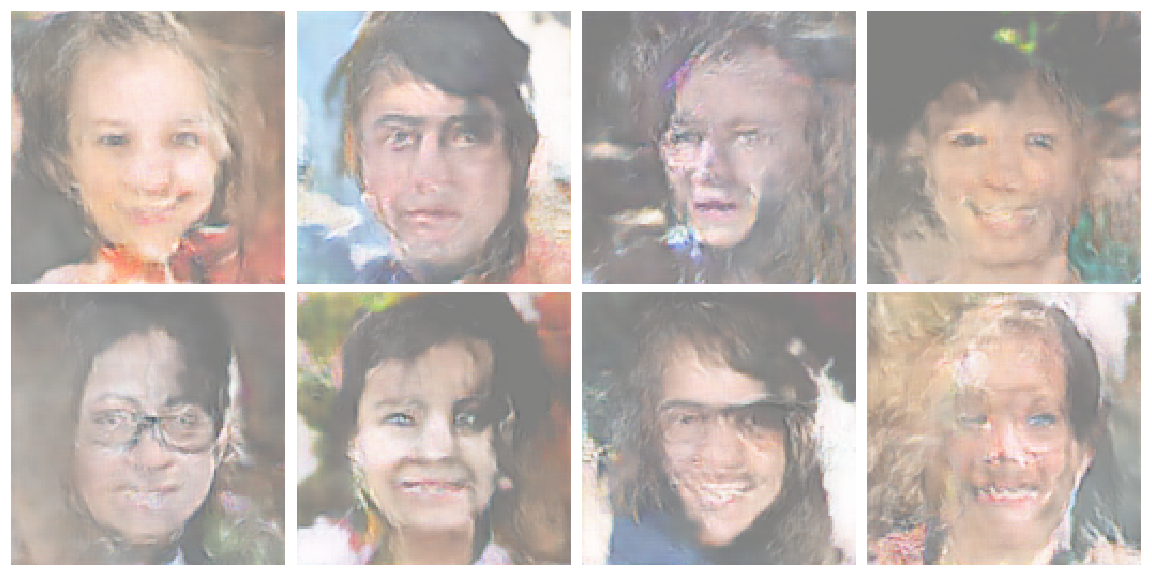
\includegraphics[width=\textwidth]{fig/dcgan/ffhq/epoch10000}
        \caption{Epoch 100000}
    \end{subfigure}
    \caption{Samples from DCGAN during training on the FFHQ dataset}
    \label{dcgan-ffhq-samples}
\end{figure}


\begin{figure}[h!]
\centering
\begin{subfigure}[b]{0.45\textwidth}
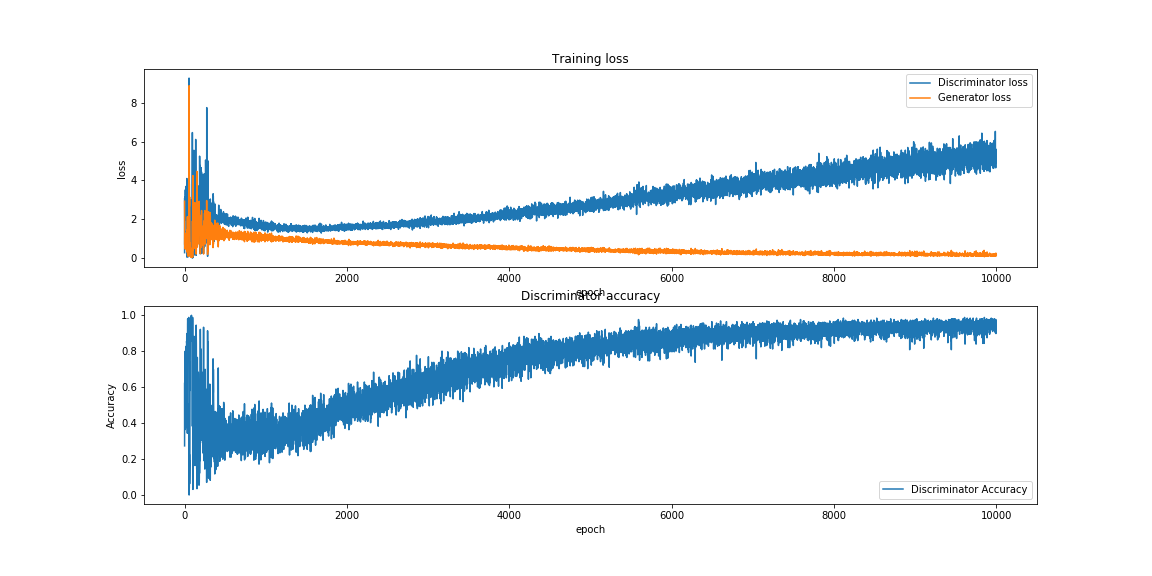
\includegraphics[width=\textwidth]{fig/dcgan/caltech/loss}
\caption{ Caltech Dataset}
\end{subfigure}
\begin{subfigure}[b]{0.45\textwidth}
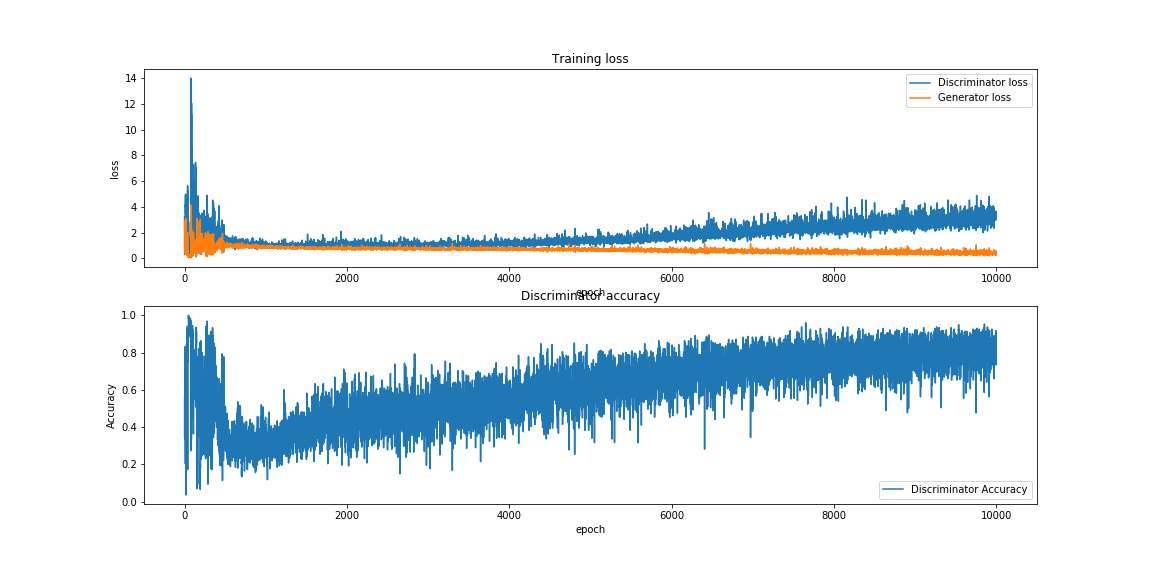
\includegraphics[width=\textwidth]{fig/dcgan/ffhq/loss}
\caption{FFHQ  Dataset}
\end{subfigure}
\caption{Loss and accuracy of the discriminator during training}
\end{figure}

\begin{figure}
    \centering
    \begin{subfigure}[b]{0.45\textwidth}
        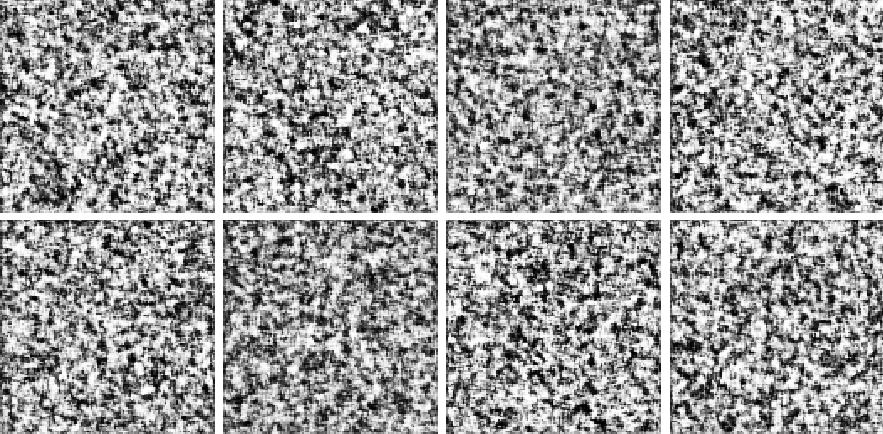
\includegraphics[width=\textwidth]{fig/dcgan/caltech/epoch0}
        \caption{Epoch 0}
    \end{subfigure}
    ~
    \begin{subfigure}[b]{0.45\textwidth}
        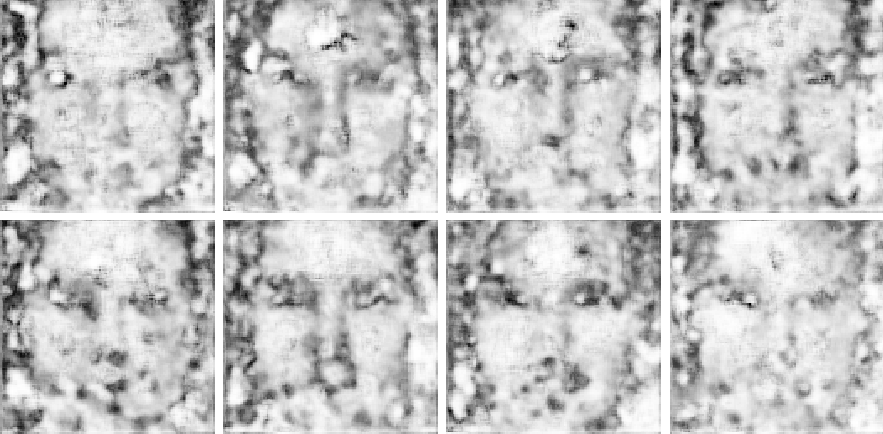
\includegraphics[width=\textwidth]{fig/dcgan/caltech/epoch200}
        \caption{Epoch 200}
    \end{subfigure}

    \begin{subfigure}[b]{0.45\textwidth}
        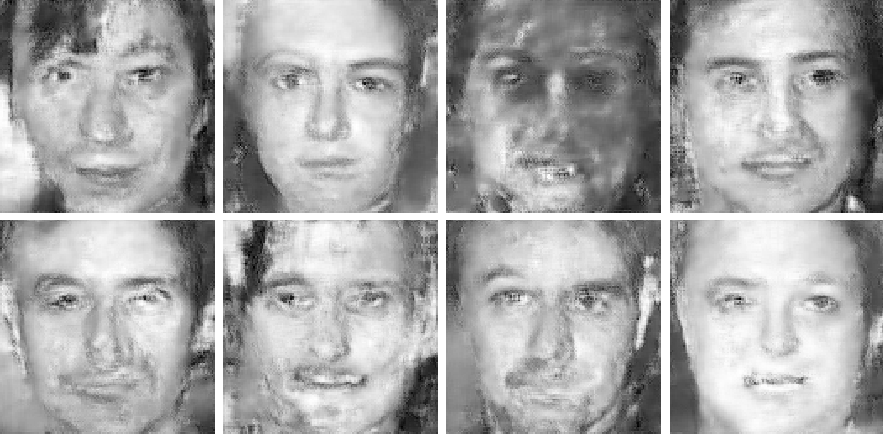
\includegraphics[width=\textwidth]{fig/dcgan/caltech/epoch2000}
        \caption{Epoch 200}
    \end{subfigure}
    ~
    \begin{subfigure}[b]{0.45\textwidth}
        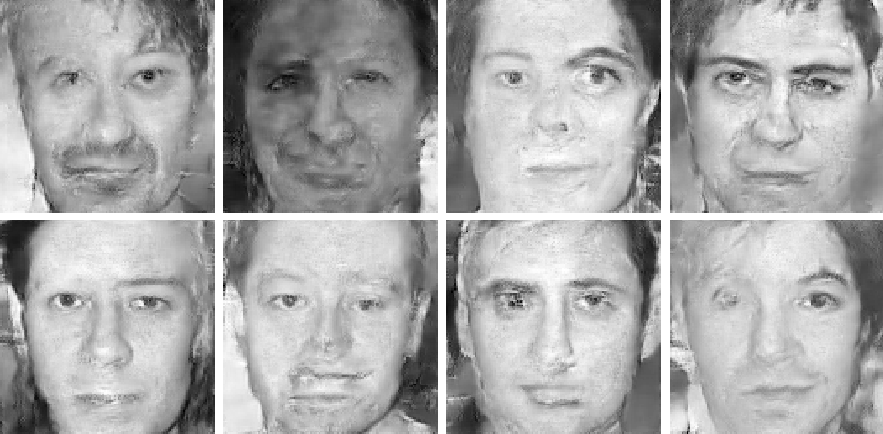
\includegraphics[width=\textwidth]{fig/dcgan/caltech/epoch4000}
        \caption{Epoch 4000}
    \end{subfigure}

    \begin{subfigure}[b]{\textwidth}
        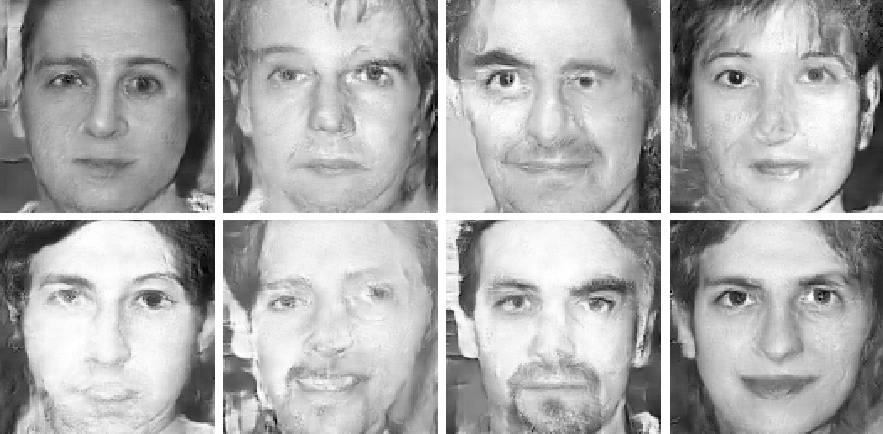
\includegraphics[width=\textwidth]{fig/dcgan/caltech/epoch10000}
        \caption{Epoch 10000}
    \end{subfigure}
    \caption{Samples from DCGAN during training on the Caltech dataset}
    \label{dcgan-caltech-samples}
\end{figure}

